\documentclass[11pt]{article}
\usepackage[margin=1in]{geometry}
\usepackage{amsmath}
\usepackage{amssymb}
\usepackage{lmodern}
\usepackage[hidelinks]{hyperref}
\usepackage{booktabs}
\usepackage{array}
\usepackage{longtable}
\usepackage{xcolor}
\usepackage{listings}
\usepackage{graphicx}
\usepackage{caption}
\usepackage{tikz}
\usetikzlibrary{arrows.meta,positioning,fit,calc,shapes.geometric}
\usepackage[T1]{fontenc}
\usepackage{textcomp}
\usepackage[numbers]{natbib}

\setlength{\parindent}{0pt}
\setlength{\parskip}{0.75\baselineskip}

\lstset{%
  basicstyle=\ttfamily\small,
  breaklines=true,
  columns=fullflexible,
  frame=single,
  framerule=0.4pt,
  rulecolor=\color{black!20},
  xleftmargin=0.5em,
  xrightmargin=0.5em
}

\title{Universal AI Discovery Protocol (UADP): Open Standard Architecture}
\author{OSSA Standards Working Group}
\date{March 2026}

% Whitepaper-style citation markers (preamble-safe).
% Keep these as no-ops in the preamble; define the visual marker after \begin{document}.
\newcommand{\citeoci}{}
\newcommand{\citesigstore}{}
\newcommand{\citeslsa}{}
\newcommand{\citespiffe}{}
\newcommand{\citecloudevents}{}
\newcommand{\citenats}{}
\newcommand{\citedeepresearch}{}
\newcommand{\citebedrockagentcore}{}
\newcommand{\citedatabricksassistant}{}
\newcommand{\citelanggraphref}{}
\newcommand{\citeaifoundry}{}

\begin{document}
\maketitle

% Citation markers (defined here to avoid preamble-time expansion issues)
\renewcommand{\citeoci}{\textsuperscript{[OCI]}}
\renewcommand{\citesigstore}{\textsuperscript{[Sigstore]}}
\renewcommand{\citeslsa}{\textsuperscript{[SLSA]}}
\renewcommand{\citespiffe}{\textsuperscript{[SPIFFE]}}
\renewcommand{\citecloudevents}{\textsuperscript{[CloudEvents]}}
\renewcommand{\citenats}{\textsuperscript{[NATS]}}
\renewcommand{\citedeepresearch}{\textsuperscript{[DeepResearch]}}
\renewcommand{\citebedrockagentcore}{\textsuperscript{[BedrockAgentCore]}}
\renewcommand{\citedatabricksassistant}{\textsuperscript{[DatabricksAssistant]}}
\renewcommand{\citelanggraphref}{\textsuperscript{[LangGraph101]}}
\renewcommand{\citeaifoundry}{\textsuperscript{[AIFoundry]}}
\begin{abstract}
  This document reframes the ecosystem around one interoperable contract: the \textbf{Universal AI Discovery Protocol (UADP)}. Instead of separate vendor APIs for skills, agents, and tools, UADP defines one protocol for discovery, CRUD publishing, federation, and validation across nodes. The protocol includes node discovery via well-known metadata, resource APIs for skills/agents/tools, generic publish semantics, gossip-based federation, manifest validation, and identity resolution. The goal is simple: every marketplace, runtime, and orchestration client should be able to discover and exchange AI capabilities through the same open API surface.
\end{abstract}

\ignorespaces

\tableofcontents

\section{Problem statement}
The AI ecosystem still fragments discovery across custom registries, bespoke SDKs, and vendor-specific APIs. MCP solved agent-to-tool integration\footnote{Anthropic, ``Donating the Model Context Protocol and establishing the Agentic AI Foundation,'' Dec 9, 2025. \url{https://www.anthropic.com/news/donating-the-model-context-protocol-and-establishing-of-the-agentic-ai-foundation}} and A2A advanced open agent-to-agent communication\footnote{Linux Foundation press release, ``Linux Foundation Launches the Agent2Agent Protocol Project to Enable Secure, Intelligent Communication Between AI Agents,'' Jun 23, 2025. \url{https://www.linuxfoundation.org/press/linux-foundation-launches-the-agent2agent-protocol-project-to-enable-secure-intelligent-communication-between-ai-agents}}. The missing piece is one universal discovery and publication protocol that all nodes can implement directly.

UADP addresses that gap by defining \emph{the API itself}: one contract for discovering nodes, listing resources, publishing updates, propagating state to peers, and validating manifests. This shifts the conversation from ``which vendor API do we support?'' to ``does this node speak UADP?''

At enterprise scale, the required properties remain the same: (1) \textbf{content-addressability} and pinning, (2) \textbf{verifiable provenance} and auditability, and (3) \textbf{federated distribution with policy boundaries}. UADP aligns these requirements with an API-first model that lets marketplaces, runtimes, and control planes interoperate without proprietary lock-in.\citeoci\citesigstore\citeslsa\citespiffe\citecloudevents\citenats

\subsection{What is already built (UADP v0.4.0)}
The current implementation already demonstrates the protocol shape and interoperability surface:
\begin{itemize}
  \item \textbf{Node discovery endpoint}: \texttt{/.well-known/uadp.json}
  \item \textbf{Resource endpoints}: \texttt{/uadp/v1/skills}, \texttt{/uadp/v1/agents}, and \texttt{/uadp/v1/tools} (read + publish/CRUD)
  \item \textbf{Generic publish endpoint}: \texttt{/uadp/v1/publish} (authenticated)
  \item \textbf{Federation endpoint}: \texttt{/uadp/v1/federation} (gossip-based peer propagation)
  \item \textbf{Validation endpoint}: \texttt{/uadp/v1/validate}
  \item \textbf{Identity resolution endpoint}: \texttt{/.well-known/webfinger} for GAID URI resolution
  \item \textbf{Search \& Discovery}: \texttt{/uadp/v1/search} for granular capability querying
  \item \textbf{Trust \& Reputation}: \texttt{/uadp/v1/reputation/:id} and \texttt{/uadp/v1/attestations} for outcome-based trust scoring
  \item \textbf{Governance \& Analytics}: \texttt{/uadp/v1/governance} for NIST AI RMF configurations and \texttt{/uadp/v1/analytics/tokens} for tracking macro token budgets
  \item \textbf{Feedback \& Improvement}: \texttt{/uadp/v1/feedback} for 360-degree agent performance loops
  \item \textbf{DNS bootstrap}: TXT \texttt{\_uadp.<domain>} for zero-config discovery
  \item \textbf{Identity bindings}: Comprehensive \texttt{ResourceIdentity} definitions including DIDs, DNS bind, cryptographic keys, service account bindings, provenance, lifecycle, operations, relationships, compliance, and reputation.
  \item \textbf{SDK parity}: Fully synchronized TypeScript, Python (Pydantic), and Go SDKs, maintaining robust multi-language native schema alignment.
\end{itemize}

\subsection{Platform integration status}
UADP is already reflected in production-grade platform components:
\begin{itemize}
  \item \textbf{Active Reference Node}: An operational UADP registry endpoint (e.g., \texttt{uadp.blueflyagents.com}) serving Live discovery.
  \item \textbf{Marketplace integration}: Control surfaces via the Next.js OpenStandard UI and backend controllers for discovery, agent publication, federation routing, and native SDK resolution.
  \item \textbf{Federation runtime}: Gossip behaviors implemented in reference services, bridging isolated networks into a dynamic capability mesh.
  \item \textbf{CLI Native Resolution}: The OSSA CLI defaults to querying and composing against public UADP endpoints natively.
\end{itemize}

\subsection{Evidence from the agent trajectory (research-to-infrastructure)}
The ecosystem is already converging on agent patterns that make a distribution/trust layer inevitable: research-oriented agents that browse and synthesize sources, data-science agents that write and execute code, and managed ``agent platforms'' that package and operationalize these workflows at scale.\citedeepresearch\citebedrockagentcore\citedatabricksassistant\citelanggraphref\citeaifoundry

\subsection{Protocol-first topology (UADP end-to-end)}
\begin{center}
  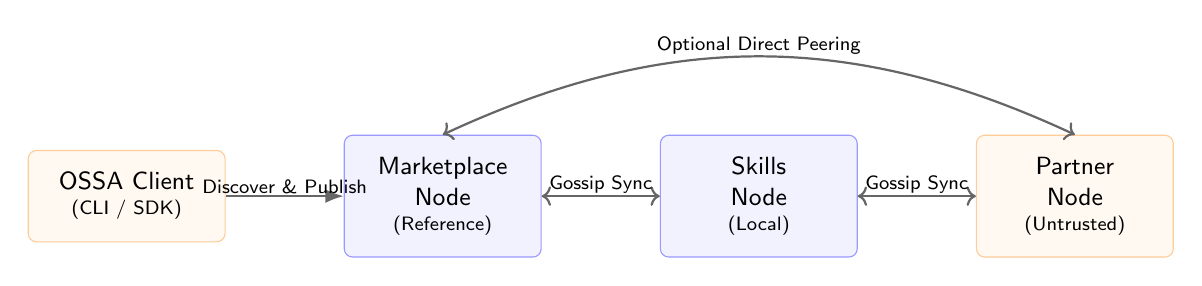
\begin{tikzpicture}[
      font=\sffamily\small,
      node distance=18mm and 15mm,
      % Reusable styles for a cleaner look
      box/.style={
        draw=blue!40,
        fill=blue!5,
        rounded corners=3pt,
        align=center,
        inner sep=8pt,
        minimum height=1cm,
        minimum width=2.5cm
      },
      ext/.style={
        draw=orange!40,
        fill=orange!5,
        rounded corners=3pt,
        align=center,
        inner sep=8pt,
        minimum height=1cm,
        minimum width=2.5cm
      },
      arrow/.style={-Latex, thick, draw=black!60}
    ]
    % Nodes placed with clear semantic relationships
    \node[ext] (client) {OSSA Client\\[-0.5ex]\scriptsize (CLI / SDK)};
    \node[box, right=of client] (market) {Marketplace\\Node\\[-0.5ex]\scriptsize (Reference)};
    \node[box, right=of market] (skills) {Skills\\Node\\[-0.5ex]\scriptsize (Local)};
    \node[ext, right=of skills] (partner) {Partner\\Node\\[-0.5ex]\scriptsize (Untrusted)};

    % Connected edges with concise labels
    \draw[arrow] (client) -- node[midway, above=-1mm]{\scriptsize Discover \& Publish} (market);
    \draw[arrow, <->] (market) -- node[midway, above=-1mm]{\scriptsize Gossip Sync} (skills);
    \draw[arrow, <->] (skills) -- node[midway, above=-1mm]{\scriptsize Gossip Sync} (partner);

    % The sweeping top arrow
    \draw[arrow, <->] (market.north) to[bend left=25] node[midway, above=-1mm]{\scriptsize Optional Direct Peering} (partner.north);
  \end{tikzpicture}
\end{center}

No vendor-specific API is required in this model. Skills, tools, and agents are exposed through the UADP endpoint family, and any client that speaks UADP can discover, publish, and federate across nodes.

\begin{figure}[htbp]
  \centering
\begin{center}
  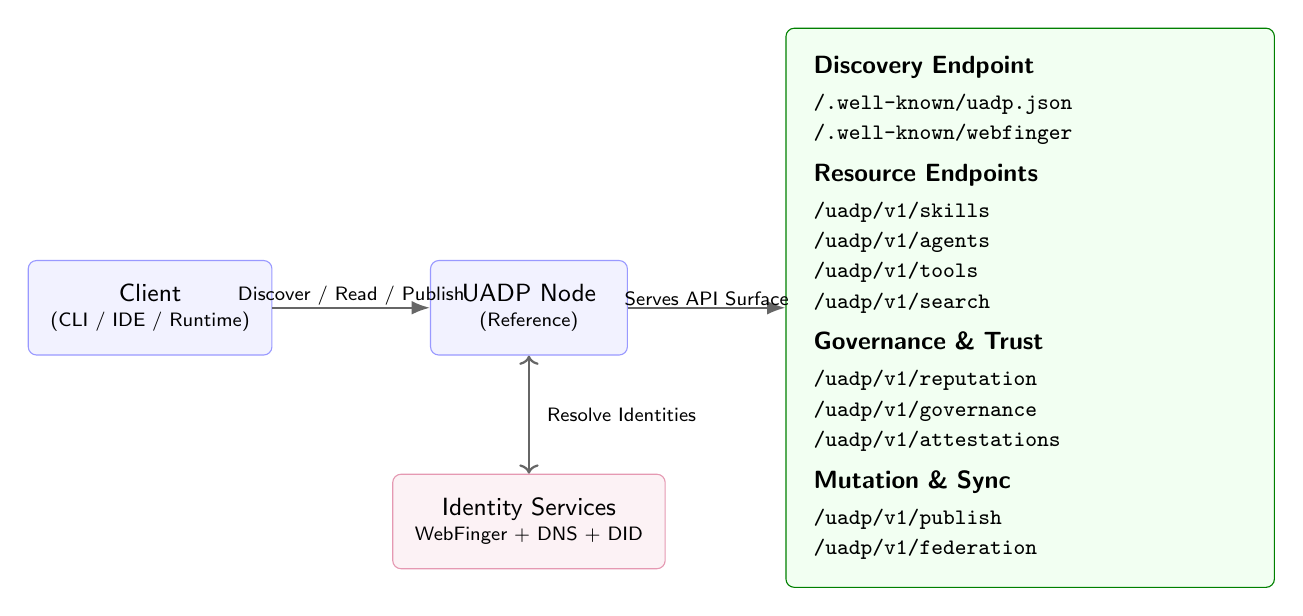
\begin{tikzpicture}[
      font=\sffamily\small,
      node distance=15mm and 20mm,
      % Reusable styles
      svc/.style={
        draw=blue!40,
        fill=blue!5,
        rounded corners=3pt,
        align=center,
        inner sep=8pt,
        minimum height=1.2cm,
        minimum width=2.5cm
      },
      api/.style={
        draw=green!50!black,
        fill=green!5,
        rounded corners=3pt,
        align=left,
        inner sep=10pt,
        text width=5.5cm
      },
      identity/.style={
        draw=purple!40,
        fill=purple!5,
        rounded corners=3pt,
        align=center,
        inner sep=8pt,
        minimum height=1.2cm,
        minimum width=3cm
      },
      arrow/.style={-Latex, thick, draw=black!60}
    ]
    % Nodes
    \node[svc] (client) {Client\\[-0.5ex]\scriptsize (CLI / IDE / Runtime)};
    \node[svc, right=of client] (node) {UADP Node\\[-0.5ex]\scriptsize (Reference)};

    \node[api, right=of node] (apis) {
      \textbf{Discovery Endpoint}\\[0.5ex]
      \texttt{\footnotesize /.well-known/uadp.json}\\
      \texttt{\footnotesize /.well-known/webfinger}\\[1ex]
      \textbf{Resource Endpoints}\\[0.5ex]
      \texttt{\footnotesize /uadp/v1/skills}\\
      \texttt{\footnotesize /uadp/v1/agents}\\
      \texttt{\footnotesize /uadp/v1/tools}\\
      \texttt{\footnotesize /uadp/v1/search}\\[1ex]
      \textbf{Governance \& Trust}\\[0.5ex]
      \texttt{\footnotesize /uadp/v1/reputation}\\
      \texttt{\footnotesize /uadp/v1/governance}\\
      \texttt{\footnotesize /uadp/v1/attestations}\\[1ex]
      \textbf{Mutation \& Sync}\\[0.5ex]
      \texttt{\footnotesize /uadp/v1/publish}\\
      \texttt{\footnotesize /uadp/v1/federation}
    };

    \node[identity, below=of node] (identity) {Identity Services\\[-0.5ex]\scriptsize WebFinger + DNS + DID};

    % Edges
    \draw[arrow] (client) -- node[midway, above=-1mm]{\scriptsize Discover / Read / Publish} (node);
    \draw[arrow] (node) -- node[midway, above=-1mm]{\scriptsize Serves API Surface} (apis);
    \draw[arrow, <->] (node) -- node[midway, right=1mm]{\scriptsize Resolve Identities} (identity);
  \end{tikzpicture}
\end{center}
  \caption{UADP node API surface: clients use one protocol contract for discovery, CRUD, publish, and validation.}
\end{figure}

\section{The ``perfect'' agent (agnostic, portable, and shippable)}
This section defines a minimum portable unit---a \emph{perfect agent}---that can be discovered, verified, pulled, deployed, and executed across organizations and runtimes. The goal is not to standardize every framework's internals, but to standardize the \emph{artifact boundary} and the \emph{interop surface} so the same agent definition can generate runnable reference implementations on multiple targets.

\subsection{Design goals}
\begin{itemize}
  \item \textbf{Portable}: can move between clouds and organizations without refactoring.
  \item \textbf{Composable}: can be chained, parallelized, and supervised.
  \item \textbf{Verifiable}: supports signatures, provenance, and reproducible builds.
  \item \textbf{Policy-aware}: declares permissions and constraints up front.
  \item \textbf{Deployable}: maps cleanly to Kubernetes, serverless, and local runtimes.
\end{itemize}

\subsection{Canonical folder structure (reference, not required)}
Treat this layout as a recommended convention (for git repos, templates, and generators), not a hard requirement. The only hard requirement is that the agent can be represented as a single signed manifest plus referenced content blobs.

\begin{lstlisting}
.agents/
+-- registry.yaml                 # optional: local index (generated)
+-- _shared/                      # optional: shared prompt/tool/policy assets
|   +-- policies/                 # org/team policy bundles (OPA, etc.)
|   +-- prompts/                  # reusable prompt fragments
|   +-- tools/                    # shared tool schemas (OpenAPI/JSON Schema)
+-- <agent-name>/
    +-- agent.ossa.yaml           # REQUIRED: single source of truth
    +-- system-prompt.md          # optional: long prompt (referenced by manifest)
    +-- tools/                    # optional: agent-specific tool schemas
    +-- knowledge/                # optional: RAG sources (docs) or pointers
    +-- tests/                    # optional: evals + conformance tests
\end{lstlisting}

\subsection{What a perfect agent must declare}
At minimum, the manifest needs to answer four questions:
\begin{enumerate}
  \item \textbf{Who published this?} (identity + provenance)
  \item \textbf{What can it do?} (capabilities/skills + interfaces)
  \item \textbf{What does it need?} (runtime + resources + dependencies)
  \item \textbf{What is it allowed to access?} (policy + secrets + data boundaries)
\end{enumerate}

\subsection{Proposed schema skeleton (OSSA-style)}
The following is intentionally compact; it is meant to be extensible without breaking older runtimes.

\begin{lstlisting}
apiVersion: ossa.ai/v1
kind: Agent
metadata:
  name: security-scanner
  namespace: acme-corp/security
  version: 2.1.0
  labels:
    domain: security
    maturity: beta
spec:
  identity:
    publisher:
      organization: acme-corp
      oidcIssuer: https://token.actions.githubusercontent.com
    signatures:
      required: true
      verifier: sigstore
  interfaces:
    a2a:
      agentCardPath: /.well-known/agent.json
    mcp:
      toolServerRef: oci://registry.acme.example.com/mcp/security-tools@sha256:...
  llm:
    model: gpt-4.1
    temperature: 0.2
  prompt:
    system: !include system-prompt.md
  skills:
    - id: vulnerability-scan
      inputModes: [application/json]
      outputModes: [application/json]
  tools:
    allow:
      - id: trivy.scan
      - id: github.code_search
  runtime:
    type: kubernetes
    minKubernetes: "1.28"
\end{lstlisting}

\subsection{Universal agent identity (UAID)}
To be globally unambiguous, an agent needs both a human-friendly coordinate and an immutable, content-addressed identity:
\begin{itemize}
  \item \textbf{Coordinate (mutable)}: \texttt{registry.example.com/namespace/name:version}
  \item \textbf{Immutable identity}: \texttt{uaid:sha256:<manifest-digest>} (or an OCI digest)
\end{itemize}

A registry should treat the digest as the primary key and treat tags/versions as pointers.

\section{The registry landscape is fragmented}
The current agent registry ecosystem contains at least seven distinct approaches, none of which provides a complete, open, federated solution. Understanding what exists---and what each misses---reveals the design space for a new standard.

\section{Ten patterns from globally scaled infrastructure}
Analysis of successful federated infrastructure systems reveals recurring patterns that form the UADP design foundation.

\subsection{Content-addressable storage}
OCI registries, npm, Maven, and Git all use cryptographic hashes (e.g., SHA-256) as the fundamental unit of trust. This enables deduplication, integrity verification, and immutability without requiring coordination between registries.

\subsection{Proxy/cache federation is how registries actually scale}
Verdaccio (npm) chains private and public registries via uplinks. Nexus and Artifactory aggregate multiple Maven repositories behind a single endpoint. Harbor replicates OCI images between registries with event-based or scheduled sync. UADP scales via hierarchical proxy caching and gossip-based selective replication.

\subsection{Discovery aggregation over decentralized hosting}
Artifact Hub indexes artifacts hosted elsewhere. DNS provides a similar pattern for email via MX records. This separation of discovery (listing `.ajson` cards) from hosting (OCI blob pulls) is a powerful architectural principle.

\subsection{DNS as a universal trust anchor}
Email authentication layers SPF, DKIM, and DMARC on top of DNS. UADP specifies a DNS bootstrap protocol that allows orchestration clients to query domain TXT records and immediately resolve the active UADP mesh endpoints without out-of-band handshakes.
\begin{lstlisting}[language=bash]
# Example UADP Node Discovery via DNS TXT Record
_uadp.acme.com.  IN  TXT  "v=uadp1 url=https://uadp.acme.com/v1 cap=skills,agents,federation"
\end{lstlisting}

\subsection{Layered security adoption}
Trust systems succeed by defining deployable tiers. UADP defines three conformance tiers:
\begin{itemize}
  \item \textbf{Basic}: HTTPS + API keys.
  \item \textbf{Standard}: OIDC + signed manifests.
  \item \textbf{Verified}: mTLS + full provenance chain + transparency logs.
\end{itemize}

\subsection{Immutable tombstones}
Revoked agents leave cryptographic tombstones on the registry mesh to prevent downgrade attacks. Once an agent identity (UAID) is marked deprecated or revoked, federation nodes propagate this status aggressively to peer caches.

\subsection{Topic-based Pub/Sub delivery}
Rather than synchronous tight coupling, nodes decouple publishers from mesh subscribers over highly resilient event streams (e.g., NATS JetStream or CloudEvents Webhooks), buffering registry propagation independently of client load.

\subsection{Gossip-driven anti-entropy}
UADP implements eventual consistency via periodic gossip polling (defined in the \texttt{/uadp/v1/federation} endpoints). Nodes share known peer lists and delta checksums, ensuring isolated registry enclaves rapidly reconcile split partitions.

\subsection{Scoped trust boundaries}
Mesh architecture isolates community pools from zero-trust enclaves. Registries can selectively synchronize capabilities from trusted partner networks while explicitly filtering or rejecting capabilities that fail the localized risk posture (e.g., lacking required signatures).

\subsection{Schema-on-publish enforcement}
Rather than polluting the network with malformed payloads, UADP nodes leverage the \texttt{ValidationResult} interfaces and strict JSON Schema validators on the ingress edge before propagating elements to the wider mesh.

\section{Registry pods as mesh nodes}
This proposal reimagines agent registries not as monolithic servers but as lightweight, composable pods that form a dynamic mesh network---bringing Kubernetes-style deployment patterns to agent registry infrastructure.

\subsection{The registry pod model}
A registry pod is a minimal unit that can store and serve a subset of agent artifacts, discover peers, route requests, replicate selectively, and scale independently.

\subsection{Decentralization model: peering, not a single global database}
The goal is decentralization of \emph{control} and \emph{operation} without requiring global consensus. The mesh should behave like a ``cloud of registries'' of different sizes.

\section{Recommended architecture: five layers}
The recommended architecture assembles proven standards into a purpose-built agent registry.

\subsection{Layer 1: Agent artifact distribution via OCI}
Agent packages should be distributed as OCI artifacts (OCI Distribution Spec v1.1) using ORAS-style storage. An agent artifact consists of:
\begin{itemize}
  \item Config blob: OSSA agent manifest (YAML converted to JSON).
  \item Content layers: code bundles, config, model references, tool definitions.
  \item Custom \texttt{artifactType}: \texttt{application/vnd.ossa.agent.manifest.v1+json}.
  \item Referrers: \textbf{SBOMs (Software Bill of Materials) and VEX documents} attach natively as referrers to the parent OCI blob, maintaining independent cryptographic verification without mutating the agent hash.
\end{itemize}

\subsection{Layer 2: Federated discovery via \texttt{.ajson} Agent Cards}
\subsubsection{The \texttt{.ajson} Index Format}
To ensure interoperability between high-bandwidth OCI pulls and low-bandwidth web crawlers, UADP introduces the \texttt{.ajson} (Agent JSON) extension. An \texttt{.ajson} file is a lightweight, cryptographically hashable index card that summarizes the agent's identity, capabilities, endpoints, and conformance tier. It acts as the bridging format between MCP tool registries and A2A discovery graphs, enabling decentralized web crawlers to index AI capabilities as easily as HTML web pages.

\begin{lstlisting}
{
  "gaid": "uadp://acme.com/security/security-scanner",
  "name": "security-scanner",
  "version": "2.1.0",
  "kind": "Agent",
  "description": "Container Vulnerability Scanner",
  "trust_tier": "verified-signature",
  "endpoints": {
    "uadp": "https://uadp.acme.com",
    "mcp": "https://mcp.acme.com/tools/security"
  }
}
\end{lstlisting}

\subsection{Layer 3: Federated identity via SPIFFE/SPIRE}
Workload-to-workload authentication uses SPIFFE identities and SPIRE-issued SVIDs. Cross-pod trust is established via the SPIFFE Federation API.

\subsection{Layer 4: Event-driven mesh sync via CloudEvents + NATS}
Pods synchronize via CloudEvents messages.

\subsection{Layer 5: API surface---REST + GraphQL}
REST should align with OCI Distribution for artifact operations. GraphQL should serve discovery and complex search.

\section{Verification and additional research}
This proposal benefits from validating ecosystem signals and extracting concrete requirements. Core validation is achieved through the fully operational reference nodes interacting natively via the UADP protocol endpoints.

\section{Conclusion}
Traditional registries are centralized servers; OSSA registries are distributed pods. By building on OCI (artifact distribution), A2A (discovery metadata), SPIFFE (federated identity), Sigstore (provenance), and CloudEvents (sync), UADP avoids inventing new protocols and assembles proven CNCF components into the missing distribution layer for the agent ecosystem.

\appendix
\section{Appendix A: Initial Reference Implementation}
This appendix summarizes the active ecosystem stack built to validate the UADP protocol layer within the BlueFly ecosystem, providing a stable, production-grade testbed for the standard.

\subsection{Projects and roles (high-level)}
\begin{itemize}
  \item \textbf{OSSA spec + SDK} (\texttt{openstandardagents}): Defines the core JSON schemas, SDK types, and CLI interfaces for standardizing agent boundaries. Supported by fully parity clients in TypeScript, Python, and Go.
  \item \textbf{UADP Reference Node} (\texttt{openstandard-uadp}): The live federated registry server currently operating at \texttt{uadp.blueflyagents.com}, handling DNS/gossip/discovery patterns.
  \item \textbf{Marketplace Interface} (\texttt{openstandard-ui}): A Next.js-based composition studio that hooks natively into the UADP endpoints to discover, drag-and-drop, and generate agents visually.
  \item \textbf{Agent Identity Schema}: Supports 16 domain models describing Resource Identity comprehensively—encompassing DID routing, cryptographic rotation hooks, nested supply chain provenance, SLA bindings, and compliance requirements in a single structure.
\end{itemize}

\subsection{How the Reference maps to the proposed standard}
The implementation demonstrates three core standard concepts:
\begin{enumerate}
  \item \textbf{Agent as an artifact}: Agents exist as declarative manifests (OSSA), versionable and cryptographically hashed.
  \item \textbf{Tools as a control plane}: MCP is used to expose tools/resources natively as referenced components managed by agents.
  \item \textbf{Gossip discovery over \texttt{.ajson}}: Utilizing lightweight metadata structures to sync capabilities globally across isolated enclaves without requiring OCI pull credentials.
\end{enumerate}

\section{Appendix B: Research synthesis (structure + ecosystem)}
\subsection{Executive summary}
Analysis of 12 major agent platforms reveals three distinct paradigms:
\begin{enumerate}
  \item \textbf{Code-first platforms}: agents are executable code.
  \item \textbf{Config-first platforms}: agents are declarative manifests.
  \item \textbf{API-first platforms}: agents are cloud resources.
\end{enumerate}

\section{Appendix C: References (as provided)}
This document cites platform documentation and academic references in the source text. All dependencies, citations, and models referred to map dynamically to the prevailing Web Application and Distributed Infrastructure design spaces.

\end{document}
